
\documentclass[12pt,a4paper,onecolumn,oneside,parskip]{memoir}
%twoside for print version
\RequirePackage[xetex]{graphicx}
\graphicspath{ {}{img/} }

\usepackage[xetex,table,xcdraw]{xcolor}

\usepackage{tabularx}

\usepackage[
breaklinks=true,colorlinks=true,
linkcolor=blue,urlcolor=blue,citecolor=blue,% PDF VIEW
%linkcolor=black,urlcolor=black,citecolor=black,% PRINT
bookmarks=true,bookmarksopenlevel=2]{hyperref}

\usepackage{geometry}
% PDF VIEW
% \geometry{total={210mm,297mm},
% left=25mm,right=25mm,%
% bindingoffset=0mm, top=25mm,bottom=25mm}
% PRINT
\geometry{total={210mm,297mm},
left=20mm,right=20mm,
bindingoffset=10mm, top=25mm,bottom=25mm}

\OnehalfSpacing
%\linespread{1.3}

\usepackage{cite}

% TABLES
\usepackage{tablefootnote}
\usepackage{booktabs}
\usepackage{pbox}
\renewcommand{\arraystretch}{1.2} 
%\renewcommand*\cmidrule{} % No table middle lines
%\renewcommand{\arraystretch}{1.5} % Additional spacing with no middle lines
%\renewcommand*\cmidrule{\hdashline[1pt/2pt]}% Dashed middle lines
\renewcommand*\cmidrule{\midrule[0.001em]} % Thin table middle lines
%\renewcommand*\cmidrule{\midrule} % Thick table middle lines

% GRAMMAR
\usepackage[rounded]{syntax}
\setlength{\grammarparsep}{4pt plus 1pt minus 1pt}

\usepackage{amsmath}
\usepackage{amssymb}

\usepackage{multicol}
\setlength{\columnsep}{1cm}

\usepackage{subcaption}
\usepackage{mathtools}

%\usepackage{floats}
\usepackage[section,above]{placeins}

% Graphs
\usepackage{tkz-berge}
\usetikzlibrary {positioning}
\definecolor {processblue}{cmyk}{0.96,0,0,0}

% Source code
\definecolor{bluekeywords}{rgb}{0.13,0.13,1}
\definecolor{greencomments}{rgb}{0,0.5,0}
\definecolor{redstrings}{rgb}{0.9,0,0}

\usepackage{listings}
\lstdefinestyle{sharpc}{language=[Sharp]C,
	showspaces=false,
	showtabs=false,
	breaklines=true,
	showstringspaces=false,
	breakatwhitespace=true,
	escapeinside={(*@}{@*)},
	commentstyle=\color{greencomments},
	keywordstyle=\color{bluekeywords}\bfseries,
	stringstyle=\color{redstrings},
	basicstyle=\ttfamily,
	morekeywords={var}
	}
%%% STYLE OF PAGES NUMBERING
%\pagestyle{companion} %\nouppercaseheads 
%\pagestyle{headings}
%\pagestyle{ruled}
%\pagestyle{plain}
%\makepagestyle{plain}
% based on companion style
\makepagestyle{hoepelman}
%\newlength{\headwidth}
\setlength{\headwidth}{\textwidth}
  %\addtolength{\headwidth}{\marginparsep}
  %\addtolength{\headwidth}{\marginparwidth}
\makerunningwidth{hoepelman}{\headwidth}
\makeheadrule{hoepelman}{\headwidth}{\normalrulethickness}
\makeheadposition{hoepelman}{flushright}{flushleft}{}{}
\makepsmarks{hoepelman}{%
  \def\chaptermark##1{\markboth{##1}{##1}}    % left mark & right marks
  \def\sectionmark##1{\markright{%
    \ifnum \c@secnumdepth>\z@
      \thesection. \ %
    \fi
    ##1}}
  \def\tocmark{\markboth{\contentsname}{\contentsname}}
  \def\lofmark{\markboth{\listfigurename}{\listfigurename}}
  \def\lotmark{\markboth{\listtablename}{\listtablename}}
  \def\bibmark{\markboth{\bibname}{\bibname}}
  \def\indexmark{\markboth{\indexname}{\indexname}}}
\makepsmarks{hoepelman}{%
  \nouppercaseheads
  \createmark{chapter}{both}{nonumber}{}{}
  \createmark{section}{right}{shownumber}{}{. \space}
  \createplainmark{toc}{both}{\contentsname}
  \createplainmark{lof}{both}{\listfigurename}
  \createplainmark{lot}{both}{\listtablename}
  \createplainmark{bib}{both}{\bibname}
  \createplainmark{index}{both}{\indexname}
  \createplainmark{glossary}{both}{\glossaryname}}
%\makeevenfoot{hoepelman}{}{}{}
%\makeoddfoot{hoepelman}{}{}{}
\makeevenhead{hoepelman}{\normalfont\bfseries\thepage}{}{\normalfont\bfseries\leftmark}
\makeoddhead{hoepelman}{\normalfont\bfseries\thepage}{}{\normalfont\bfseries\leftmark}
%\makeoddhead{hoepelman}{\normalfont\bfseries\rightmark}{}{\normalfont\bfseries\thepage}

\pagestyle{hoepelman}

%%% CHAPTER'S STYLE
\makeatletter
\newcommand\thickhrulefill{\leavevmode \leaders \hrule height 1ex \hfill \kern \z@}
\setlength\midchapskip{10pt}
\makechapterstyle{VZ14}{
\renewcommand\chapternamenum{}
\renewcommand\printchaptername{}
\renewcommand\chapnamefont{\Large\scshape}
\renewcommand\printchapternum{%
\chapnamefont\null\thickhrulefill\quad
\@chapapp\space\thechapter\quad\thickhrulefill}
\renewcommand\printchapternonum{%
\par\thickhrulefill\par\vskip\midchapskip
\hrule\vskip\midchapskip
}
\renewcommand\chaptitlefont{\Huge\scshape\centering}
\renewcommand\afterchapternum{%
\par\nobreak\vskip\midchapskip\hrule\vskip\midchapskip}
\renewcommand\afterchaptertitle{%
\par\vskip\midchapskip\hrule\nobreak\vskip\afterchapskip}
}
\makeatother
\chapterstyle{VZ14}


%%% STYLE OF SECTIONS, SUBSECTIONS, AND SUBSUBSECTIONS
\setsecheadstyle{\Large\bfseries\sffamily\raggedright}
\setsubsecheadstyle{\large\bfseries\sffamily\raggedright}
\setsubsubsecheadstyle{\bfseries\sffamily\raggedright}


% Custom commands
\newcommand\textlcsc[1]{\textsc{\MakeLowercase{#1}}}

\newcommand{\tablelist}[1]{%
%\tightlist%
\begin{itemize}[nosep]%
#1%
\end{itemize}%
\vspace{-\baselineskip}\mbox{}}
%\usepackage[utf8]{inputenc}
\usepackage[T1]{fontenc}
\usepackage{microtype}
%\usepackage{fontspec}

%Default: computer modern

% 
%\usepackage{kpfonts}

% Times-like
%\usepackage{newtxtext}
%\usepackage{newtxmath}

% Times-like
%\usepackage{mathptmx}
%\usepackage{courier}

%Calibri
%\setmainfont{Calibri}

% Palatino
%\usepackage{newpxtext}
%\usepackage{newpxmath}

%\usepackage{libertine}
%\usepackage[libertine]{newtxmath}

\usepackage[scaled]{helvet}
\renewcommand\familydefault{\sfdefault}
\usepackage{sansmath}

\maxsecnumdepth{subsection} % chapters, sections, and subsections are numbered
\maxtocdepth{subsection} % chapters, sections, and subsections are in the Table of Contents

\newcommand{\todo}[1]{\textbf{TODO: #1}}
\newcommand{\ignore}[1]{}
\newcommand{\f}[1]{\texttt{#1}}
\newcommand{\key}[1]{\textbf{#1}}
\newcommand{\rf}[1]{\textsc{\lowercase{#1}}}
\newcommand{\noparskip}[1]{{\parskip=0pt
#1
}}
\newcommand*{\rom}[1]{\expandafter\@slowromancap\romannumeral #1@}

\nonzeroparskip

\begin{document}

\thispagestyle{empty}
\onecolumn
{%%%
\sffamily
\centering

~\vspace{\fill}

{\huge \bfseries
Inter-cell Spreadsheet Refactoring and Parsing Spreadsheet Formulas
}

\vspace{2.0cm}

by

\vspace{2.0cm}

{\LARGE
David Jonathan Hoepelman
}

\vspace{3.0cm}

\textlcsc{Master Thesis} \\
\today

\vspace{2.5cm}

For obtaining the degree of \\
Master of Science \\
in Computer Science - Software Technology \\

\vspace{0.5cm}

Faculty Electrical Engineering, Mathematics and Computer Science (EEMCS)\\
Delft University of Technology

\vspace{1.5cm}


\includegraphics{tudelft}
\hspace{0.5cm}
%
\includegraphics[height=8mm]{serg}
%\hspace{0.5cm}

\includegraphics[height=8mm]{spreadsheet-lab}
\hspace{0.5cm}

\vspace{\fill}

}

\cleardoublepage

%%%---%%%---%%%---%%%---%%%---%%%---%%%---%%%---%%%---%%%---%%%---%%%---%%%
\tableofcontents*

\clearpage
%\twocolumn

%%%---%%%---%%%---%%%---%%%---%%%---%%%---%%%---%%%---%%%---%%%---%%%---%%%
%%%---%%%---%%%---%%%---%%%---%%%---%%%---%%%---%%%---%%%---%%%---%%%---%%%

\chapter{Introduction}

Like all people, I sometimes get asked what I do for a living.
When I tell someone I am writing my master thesis in Computer Science, their eyes start to glaze over as they anticipate some explanation peppered with terms they will not understand about 
I then tell them my thesis is about spreadsheets and ask if they have ever worked with Excel, and nearly everyone who has ever worked in business or research has.
Nearly everyone has a horror story about that one unmaintainable spreadsheet that they had to work on, or that day their reporting system broke down because 2009 turned into 2010 and the spreadsheet only looked at the last digit.

This anecdotal evidence is mirrored in research.
Panko \cite{panko2006facing} estimates that 80\% to 95\% of businesses use spreadsheets in one of their processes.
Furthermore, almost all spreadsheets contain at least one error and 1 to 5\% of spreadsheet cells contains an error according to Panko \cite{panko1998we}.
Spreadsheets perform roles very similar to software in that they perform business-critical roles, are inherited throughout the organization and maintained by different users and accrue technical dept during and after the initial development period \cite{panko1998we}.
In short, spreadsheets can be classified as programs, and spreadsheet creators as end-user programmers.

This view, "spreadsheets are code", could be the one-sentence summary of the ideology of the Spreadsheet Lab, which is a part of the TU Delft Software Engineering Research Group (SERG).
Using this view as a baseline, the group has tried to translate tried and proven software engineering methods to the spreadsheet domain so that they could be used to improve spreadsheets, spreadsheet development practices and help spreadsheet programmers.
As part of this effort, a spreadsheet formula refactoring tool called BumbleBee was developed by Hermans and Dig \cite{hermans2014bumblebee}.
This tool allows a formula to be transformed into another by defining a transformation rule, which works very similar to a pattern or regular expression replacement in a text editor.

However this approach has the downside that it can only considers one formula, and not the spreadsheet as a whole.
This leads to a lack of power to implement all spreadsheet refactorings, such as those implemented by Badame and Dig \cite{badame2012refactoring} in earlier work.
I joined the group to extend the capabilities of BumbleBee so that it could take context into account when performing refactorings, and implement more refactorings in BumbleBee.

\begin{figure}
\centerfloat
\begin{subfigure}[c]{0.1\textwidth}
\f{=1+2+3}
\end{subfigure}
\begin{subfigure}[c]{0.08\textwidth}
$\xrightarrow[Ch.~\ref{chapter:parsing}]{Parsing}$
\end{subfigure}
\begin{subfigure}[c]{0.17\textwidth}
\begin{tikzpicture}[-latex ,auto ,node distance =1.3 cm and 0.5cm ,on grid , semithick,
,
state/.style ={ circle ,top color =white ,
draw, minimum width =0.75 cm}]
\node[state] (RootPlus) {$+$};
\node[state] (SecondPlus) [below left=of RootPlus] {$+$};
\node[state] (Input1) [below left=of SecondPlus] {1};
\node[state] (Input2) [below right=of SecondPlus] {2};
\node[state] (Input3) [below right=of RootPlus] {3};

\path (RootPlus) edge node {} (Input3);
\path (RootPlus) edge node {} (SecondPlus);
\path (SecondPlus) edge node {} (Input1);
\path (SecondPlus) edge node {} (Input2);
\end{tikzpicture}
\end{subfigure}
\begin{subfigure}[c]{0.14\textwidth}
$\xrightarrow[Ch.~\ref{sec:implementingrefactorings}]{Refactoring}$
\end{subfigure}
\begin{subfigure}[c]{0.17\textwidth}
\begin{tikzpicture}[-latex ,auto ,node distance =1.3 cm and 0.5cm ,on grid , semithick,
,
state/.style ={ circle ,top color =white ,
draw, minimum width =0.75 cm}]
\node[state] (Root) {$F$};
\node[state] (11) [below left=of Root] {\tiny{\f{SUM}}};
\node[state] (12) [below right=of Root] {[]};
\node[state, node distance = 1.3cm and 0.85cm] (21) [below left =of 12] {1};
\node[state, node distance = 1.32cm and 0.85cm] (22) [below =of 12] {2};
\node[state, node distance = 1.3cm and 0.85cm] (23) [below right=of 12] {3};

\path (Root) edge node {} (11);
\path (Root) edge node {} (12);
\path (12) edge node {} (21);
\path (12) edge node {} (22);
\path (12) edge node {} (23);
\end{tikzpicture}
\end{subfigure}
\begin{subfigure}[c]{0.1\textwidth}
$\xrightarrow[Ch.~\ref{sec:printing}]{Printing}$
\end{subfigure}
\begin{subfigure}[c]{0.145\textwidth}
\f{=SUM(1,2,3)}
\end{subfigure}
\caption{Overview of refactoring process}
\label{fig:refactoring-process}
\end{figure}

After the initial literature research I started implementing refactorings, but encountered a fundamental problem in doing so.
The standard way of implementing refactorings, illustrated in Figure \ref{fig:refactoring-process}, is by parsing the source code to an Abstract Syntax Tree (AST), which represents the structure of the program.
This AST can then be manipulated into the desired form, after which it can be converted back to source code (this is called printing or pretty-printing).
While BumbleBee contained a home-grown parser, I found a range of formulas that were either not parsable, or parsed into an incorrect AST.
This made me refocus the purpose of my thesis into making a better parser for Excel formulas, as this would not only be very useful for implementing refactorings but would be beneficial to all future spreadsheet research projects.

\section{About this thesis}

\subsection{Contribution}

The contributions of this thesis are twofold. Firstly there is the stand-alone parser for Excel formulas called XLParser, which is open-source and available online\footnote{\url{https://github.com/spreadsheetlab/XLParser}}. The parser was tested on over a million formulas and failed to parse merely two formulas.
Details of this parser are published by Aivaloglou, Hoepelman and Hermans \cite{xlparser}.
This paper is partially re-used in this thesis report, and the parts re-used are my contribution to the paper.

The second contribution is an improved version of BumbleBee, which implements the refactorings described in Chapter \ref{chapter:implementingrefactorings}: \rf{Extract Formula}, \rf{Inline Formula}, \rf{Group References} and \rf{Introduce Conditional Aggregate}.
BumbleBee is also available online\footnote{TODO: URL Bumblebee.}.

\subsection{Attribution}

This thesis was performed at the TU Delft Spreadsheet Lab, and is partially based on a collaborative effort in that group.
During this thesis the Excel Formula parser XLParser was developed, and a paper describing it was accepted into the 15th IEEE International Working Conference on Source Code Analysis and Manipulation (SCAM 2015): \emph{A Grammar for Spreadsheet Formulas Evaluated on Two Large Datasets} by Efthimia Aivaloglou, David Hoepelman and Felienne Hermans \cite{xlparser}.
This paper is attached verbatim as published in appendix \ref{appendix:xlparser}.
Chapter \ref{chapter:anatomy} is based on section \rom{2} of the paper, and was primarily written by the thesis author.
Chapter \ref{chapter:parser}  is an updated and extended version of section \rom{3} of the paper, and was primarily written by the thesis author with contributions from Efthimia Aivaloglou, except for section \ref{sec:parserevaluation}, which is a summary of section \rom{4} of the paper which was primarily written by Efthimia Aivaloglou, who also performed the evaluation.

The grammar implementation (XLParser) was primarily done by the thesis author, but the implementation is based on the previous (un-named) parser which was primarily developed by Efthimia Aivalgoglou and Felliene Hermans.
The tool used to evaluate XLParser, which extracts formulas from spreadsheet files, was developed as part of Infotron B.V.\footnote{\url{http://www.infotron.nl/}}, with many authors. The thesis author did not contributo to this tool.

\subsection{Outline}

A passing knowledge of Excel and more in-depth knowledge of Excel formulas is needed to read the rest of this thesis, which is bundled in chapter \ref{chapter:anatomy} "\nameref{chapter:anatomy}".
Chapter \ref{chapter:previouswork} details previous and related work on spreadsheet refactoring.
In chapter \ref{chapter:candidaterefactorings} potential spreadsheet refactorings which were not yet implemented in BumbleBee are identified.

The Chapters thereafter describe the implementation of the spreadsheet refactorings.
Chapter \ref{chapter:parsing} covers how XLParser parses spreadsheet formulas and why it was designed as it was.
Chapter \ref{chapter:implementingrefactorings} describes how spreadsheet refactorings are performed and the implementation details of the new refactorings.

\todo{Meer zodra thesis wat meer vlees heeft}

\clearpage
\section{Timeline and decisions taken}

\begin{tabularx}{\textwidth}{lX}
\toprule
December 2014 & Literature study on refactoring, refactoring spreadsheets, converting spreadsheets to programs. \\
& Thesis topic selection. \\
January 2015 & Studied practicality of generic spreadsheet refactoring language based on Bumblebee transformation language, deemed inviable. \\
& Gathered existing refactorings from spreadsheet literature and translated Fowler refactorings. \\
& Decided which refactorings to initially implement \\
& Familiarization with existing BumbleBee code \\
February 2015 & Implementing \rf{Inline Formula} \\
& Extended Bumblebee and parser to account for sheet and file names \\
March 2015 & Implementing \rf{Extract formula} \\
& Writing of paper "End user programming" \todo{} \\
April 2015 & Writing of paper "End user programming" \todo{} \\
& Various improvements to parser \\
May 2015 & Decision to rewrite parser to solve several fundamental problems \\
& Start work on XLParser \\
& Implementing \rf{Introduce (Conditional) Aggregate} \\
& Implementing \rf{Group references} \\
June 2015 & Continued work on XLParser: Initial release \\
& Writing of XLParser paper \\
July 2015 & Changing of refactoring UI to context-aware right-click menu, similar to IDE's \\
August 2015 & Continued work on XLParser: Several fixes to XLParser parse trees \\
& Camera-ready adjustment of XLParser paper \\
& Constructed demo application\footnote{\url{http://xlparser.perfectxl.nl/demo/}} for XLParser which shows the parse trees. \\
September 2015 & Continued work on XLParser: Adding structured references, file paths \\
& Porting BumbleBee and refactorings to XLParser-based implementations \\
\bottomrule
\end{tabularx}

\chapter{Previous and related work}
\label{chapter:previouswork}

\section{Refactoring}

\section{The BumbleBee spreadsheet refactoring suite}

\section{Other spreadsheet refactoring efforts}

%\chapter{Spreadsheet anatomy}
\chapter{Anatomy of spreadsheets and spreadsheet formulas}
\label{chapter:anatomy}

\noindent
\begin{figure}[h]
\centerfloat
\fbox{
\begin{subfigure}[c]{0.1\textwidth}
\centering
\vspace{3em}
\f{=1+2+3}
\vspace{3em}
\end{subfigure}
}
\begin{subfigure}[c]{0.08\textwidth}
$\xrightarrow{Parsing}$
\end{subfigure}
\begin{subfigure}[c]{0.17\textwidth}
\begin{tikzpicture}[-latex ,auto ,node distance =1.3 cm and 0.5cm ,on grid , semithick,
,
state/.style ={ circle ,top color =white ,
draw, minimum width =0.75 cm}]
\node[state] (RootPlus) {$+$};
\node[state] (SecondPlus) [below left=of RootPlus] {$+$};
\node[state] (Input1) [below left=of SecondPlus] {1};
\node[state] (Input2) [below right=of SecondPlus] {2};
\node[state] (Input3) [below right=of RootPlus] {3};

\path (RootPlus) edge node {} (Input3);
\path (RootPlus) edge node {} (SecondPlus);
\path (SecondPlus) edge node {} (Input1);
\path (SecondPlus) edge node {} (Input2);
\end{tikzpicture}
\end{subfigure}
\begin{subfigure}[c]{0.14\textwidth}
$\xrightarrow{Refactoring}$
\end{subfigure}
\begin{subfigure}[c]{0.17\textwidth}
\begin{tikzpicture}[-latex ,auto ,node distance =1.3 cm and 0.5cm ,on grid , semithick,
,
state/.style ={ circle ,top color =white ,
draw, minimum width =0.75 cm}]
\node[state] (Root) {$F$};
\node[state] (11) [below left=of Root] {\tiny{\f{SUM}}};
\node[state] (12) [below right=of Root] {[]};
\node[state, node distance = 1.3cm and 0.85cm] (21) [below left =of 12] {1};
\node[state, node distance = 1.32cm and 0.85cm] (22) [below =of 12] {2};
\node[state, node distance = 1.3cm and 0.85cm] (23) [below right=of 12] {3};

\path (Root) edge node {} (11);
\path (Root) edge node {} (12);
\path (12) edge node {} (21);
\path (12) edge node {} (22);
\path (12) edge node {} (23);
\end{tikzpicture}
\end{subfigure}
\begin{subfigure}[c]{0.1\textwidth}
$\xrightarrow{Printing}$
\end{subfigure}
\fbox{
\begin{subfigure}[c]{0.145\textwidth}
\centering
\vspace{3em}
\f{=SUM(1,2,3)}
\vspace{2em}
\end{subfigure}
}
\caption{This chapter details the properties and syntax of spreadsheets and formulas strings.}
\end{figure}

\todo{Introductie van dit chapter: "Er is een goed begrip nodig van spreadsheets, omdat ..."}

The most widely used spreadsheet system is Microsoft Office Excel, by a large margin.
Two less-popular but still common implementation are Openoffice.org and Libreoffice Calc (which evolved from the same product and thus have largely identical semantics) and Google Docs Sheets, a web-based collaborative spreadsheet program. \todo{Markaandeel van deze implementaties}.
When referencing "all" spreadsheet programs, the previous three common implementations are referenced.

Although exotic forms of spreadsheets are available and have been researched, all currently widely used implementation use the following model:
\begin{itemize}
\item A single spreadsheet \key{file} corresponds to a single (\key{work})\key{book}.
\item A workbook can contain any number of (\key{work})\key{sheets}.
\item A sheet consists of a \key{two-dimensional grid} (table) of \key{cells}.
\item A vertical unit in the grid is called a \key{column} and a horizontal unit a \key{row}.
Rows are numbered sequentially top-to-bottom starting at 1, while columns are numbered left-to-right alphabetically, i.e. base-26 using A to Z as digits.
A column or row can also mean all cells contained in that column or row.
\item A \key{cell} can contain a \key{constant value} of any type, a calculation called a \key{formula} or a matrix calculation called an \key{array formula}.
\item An (array) formula can \key{reference} other cells to use their values. When the value of a referenced cell changes, this new value is propagated and the dependent formula values are recalculated.
\end{itemize}

\begin{figure}
\centerfloat
\begin{subfigure}[b]{0.45\textwidth}
\centering
\scalebox{0.71}{
\begin{tikzpicture}[-latex ,auto ,node distance =1.3 cm and 1.8cm ,on grid , semithick,
,
state/.style ={ circle ,top color =white ,
draw, minimum width =0.9 cm}]
\node[state] (Input3) {3};
\node[state] (Input5) [below=of Input3] {5};
\node[state] (Plus) [right=of Input5] {$+$};
\node[state] (Input2) [below=of Input5] {2};
\node[state] (Times) [below right=of Plus] {$\times$};
\node[state] (Output) [right=of Times] {\small{\texttt{out}}};
\path (Input3) edge [right] node[right] {} (Plus);
\path (Input5) edge [right] node[right] {} (Plus);
\path (Plus) edge [right] node[right] {} (Times);
\path (Input2) edge [right] node[right] {} (Times);
\path (Times) edge [right] node[right] {} (Output);
%\path (A) edge [loop left] node[left] {$1/4$} (A);
%\path (C) edge [bend left =25] node[below =0.15 cm] {$1/2$} (A);
%\path (A) edge [bend right = -15] node[below =0.15 cm] {$1/2$} (C);
%\path (A) edge [bend left =25] node[above] {$1/4$} (B);
%\path (B) edge [bend left =15] node[below =0.15 cm] {$1/2$} (A);
%\path (C) edge [bend left =15] node[below =0.15 cm] {$1/2$} (B);
%\path (B) edge [bend right = -25] node[below =0.15 cm] {$1/2$} (C);
\end{tikzpicture}
}
\caption{Dataflow program}
\end{subfigure}
\hspace{0.05\textwidth}
\begin{subfigure}[b]{0.45\textwidth}
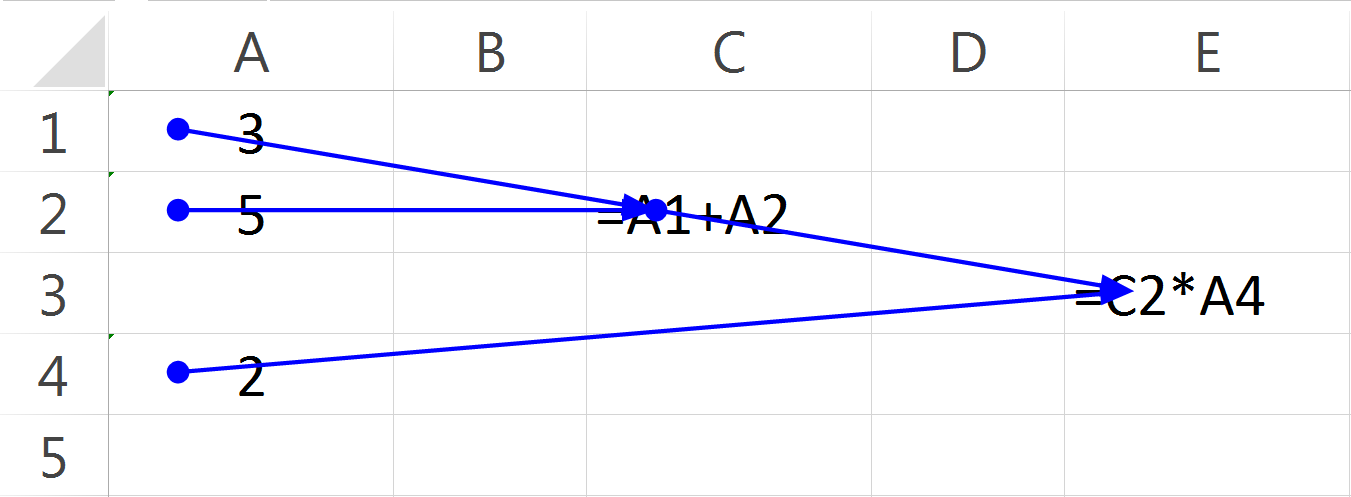
\includegraphics[width=\textwidth]{anatomy/dataflow-program-excel-implementation}
\caption{Spreadsheet implementation}
\end{subfigure}
\caption{An example dataflow program and its spreadsheet implementation}
\label{fig:dataflow-example}
\end{figure}

This model is a variation of the dataflow programming model.
A dataflow program is a directed graph, where data flows between operation in nodes along the graphs edges.
In spreadsheets, cells represent the nodes of a dataflow program and edges are represented by references.
An example dataflow program and its spreadsheet implementation can be seen in Figure \ref{fig:dataflow-example}.

The spreadsheet model is Turing complete, as proven by an Excel 2010 implementation of a Turing machine \cite{ExcelTuringComplete}.

\section{Formulas}

Currently two major formula languages exist in spreadsheets. The first is the Office Open XML spreadsheet language which is a standarization of the Excel language, which is currently used by Microsoft Excel.
The second is OASIS OpenDocument OpenFormula, which is part of the OpenDocument format which is based on the OpenOffice.org format.
Google Sheets claims to implement OpenFormula, but has some differences.
Both languages are very similar and this section covers both unless otherwise noted.

Formulas consist of expressions which can contain constant values, \key{function calls} and \key{operators} and, most importantly, \key{references} to other cells.
A cell is identified as a formula cell because all formulas must start with the equals sign \f{=}.

\subsection{Function calls and operators}

Function calls are performed similar to other programming languages by starting with the function name, followed by the arguments in parentheses, separated by a comma.
All spreadsheet implementations provide a range of built-in functions, and in most spreadsheet implementations it is possible to define new functions yourself.
However in current implementations this is not done directly inside the spreadsheet, and uses an alternate programming language.
In Microsoft Excel and Libreoffice this is done with a variant of the BASIC programming language, while in Google Sheets this is done with Javascript.
A way for the user to define functions in the spreadsheet intself has been proposed by Jones \cite{jones2003user}, but as of now has not been implemented in mainstream spreadsheet programs yet.

The operators \f{+ - * / = >= <= < >} and \f{<>} (inequality) can be used according to their usual semantics.
\f{+} and \f{-} are available both unary (\f{=-1}) and binary (\f{=1-1}).
Additionally the \f{\%} unary operator is defined to transform a number into a percentage (divining it by 100), \f{\^} is the exponentiation operator and \f{\&} is the text concatenation operator.

Spreadsheet program contain three fairly unique binary operators, the semantics of whichare detailed in section \ref{sec:references}.
Firstly there is the range operator \f{:} then the union operator (\f{,} in Excel and \f{\textasciitilde} in OpenFormula) and lastly the intersection operator (\f{\char32} in Excel and \f{!} in OpenFormula).
Note that OpenFormula diverges from the Excel syntax, possibly because the comma already is used in other places in the language and a single space as an operator is highly unusual.
The Excel characters for the operators will be used from now on.

\subsection{References}
\label{sec:references}
References are the core component of spreadsheets.
The value of any cell can be used in a formula by concatenating its column and row number, producing a reference like \f{B5}.
This is called A1-style referencing and is by far the most comment in modern spreadsheet implementations.
If the value of a cell changes, this new value will be propagated to all formulas that use it.

When copying a cell to another cell by default references will be adjusted by the offset, for example copying \f{=A1} from cell B1 to C2 will cause the copied formula to become \f{=B2}.
This can be prevented by making the reference absolute by prepending a \f{\$} to the column index, row index or both.
The formula \f{=\$A\$1} will remain the same on copy while \f{=\$A1} will still have its row number adjusted when copied, as ilustrated in Figure \ref{fig:copy-modifiers}.

\begin{figure}
\centerfloat
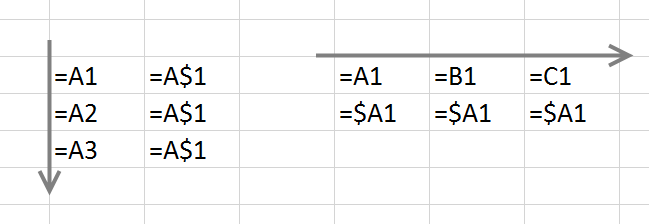
\includegraphics[width=0.5\textwidth]{anatomy/copying}
\caption{Different copy-paste behavior depending on \f{\$} modifier, copy-direction is given by the arrow.}
\label{fig:copy-modifiers}
\end{figure}


\subsection{Ranges}
References can also be \emph{ranges}, which are collections of cells.
Ranges can be constructed by three operators: the range operator \f{:}, the union operator \f{,} (a comma) and the intersection operator \f{\char32} (a space).
The range operator \f{:} creates a rectangular range with the two cells as top-left and bottom-right corners, so \f{=SUM(A1:B10)} will sum all cells in columns A and B with row number 1 through 10.
The range operator is also used to construct ranges of whole rows or columns, for example \f{3:5} is the range of the complete rows three through five, and \f{A:D} is the range of columns A through D.
The union operator, which is different from the mathematical union as duplicates are allowed, combines two references, so \f{A1,C5} will be a range of two cells, \f{A1} and \f{C5}.
Lastly the intersection operator takes only the cells which are in both arguments, \f{=A:A 5:5} will thus be equivalent to \f{=A5}.

A user can also give a name to any collection of cells, thus creating a \emph{named range} which can be referenced in formulas by name.
For example one can give the name \f{TAX\_RATE} to cell \f{A2} and then use this in a formula: \f{=C3+C3*TAX\_RATE} instead of \f{=C3+C3*\$A\$2}.

\subsection{Structured References}

A recent, Excel 2007, addition to the Excel formula language are structured (table) references.
To use this feature, a table can be given a name and must have headers.
One can then reference a column in the table by entering \f{TableName[ColumnName]}.
Inside the square brackets reference operators can be used to construct more complex references, \f{TableName[Column1,Column4]} references two columns.

There is no way to reference a specific row, except the current row, for example if a formula is placed in \f{A3} it can only reference row number 3.
The \f{\#This Row} keyword and the \f{@} operator are used for this: \f{TableName[\#This Row]} and \f{TableName[@]} both reference the current row number in the provided table, and \f{TableName[@ColumnName]} references the cell in the provided column of the current row number.

This feature is meant to make formulas easier to read, by references in a formula like \f{=SUM(F1:F10)-SUM(I1:I10)} with human-readable names like \f{=SUM(Budget[Revenue]) - SUM(Budget[Expenses])}.

\subsection{R1C1 reference style}

An alternate style called R1C1 as opposed to the above A1 style exists, but it is very rarely seen or used by users.
In R1C1 reference style one specifies either the offset to a cell between square brackets or its concrete location.
In R1C1 style \f{R[4]C[-2]} means the cell two columns to the left and four rows down, while \f{R2C2} refers to cell B2.
The biggest advantage of R1C1 is that it causes identical formulas to be the same even when they operate on different cells or data because of their position, illustrated in Figure \ref{fig:r1c1comp}.
These properties make R1C1 useful as an internal representation in spreadsheet implementations.

\begin{figure}
\centerfloat
\begin{subfigure}[t]{0.35\textwidth}
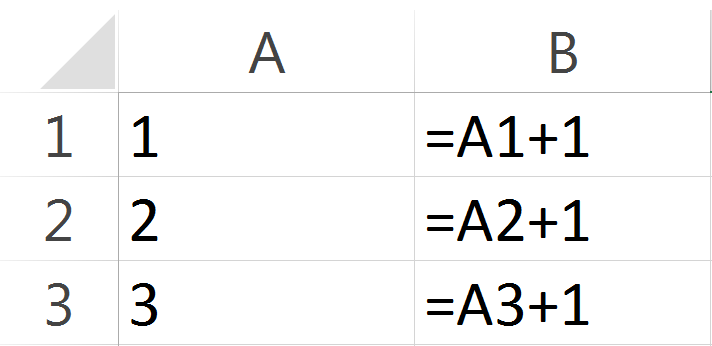
\includegraphics[width=1\textwidth]{anatomy/r1c1comp-a1}
\caption{A1-style formulas}
\end{subfigure}
\hspace{0.1\textwidth}
\begin{subfigure}[t]{0.35\textwidth}
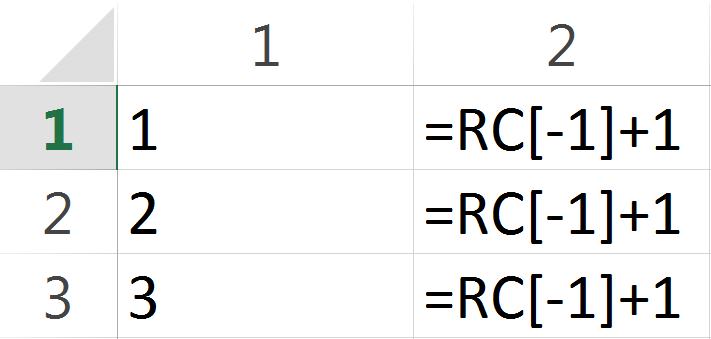
\includegraphics[width=1\textwidth]{anatomy/r1c1comp-r1c1}
\caption{R1C1-style formulas}
\end{subfigure}
\caption{A1 vs R1C1 behavior on identical formulas with respect to cell position}
\label{fig:r1c1comp}
\end{figure}

\subsection{Non-local references}
\label{subsection:ExternalRefsDDE}

References refer to cells or ranges in the same sheet as the formula by default, but this can be modified with a prefix. A non-local reference consists a prefix indicating the location, followed by an exclamation mark, followed by the actual reference.

The most common use case is to reference another sheet in the same workbook, where the prefix is simply the sheet name: \f{=Sheetname!A1}.
Sheet names can also be between single quotes if they contain special characters: \f{='Sheetname with space'!A1}. 
References to external spreadsheet files are also possible, which is done by providing the file name in between square brackets and optionally the file path: \f{=[Filename]Sheetname!A1} or \f{='C:{\textbackslash}Path{\textbackslash}[Filename]Sheet'!A1}.
A peculiar type of prefix are those that indicate multiple sheets: \f{=Sheet1:Sheet10!A1} means A1 in Sheet1 through Sheet10.

In Windows versions of Microsoft Excel formulas can also call external programs through Dynamic Data Exchange (DDE).
DDE links are a special case of references, used for receiving data from other applications.
They take the form of \f{=Program|Topic!Arguments}, e.g. \f{=Database|TableA!Column1}.

\subsection{Case sensitivity}

Formulas are case-insensitive outside of the trivial case of string literals.
Identifiers have a canonical capitalization, and while user can type the identifier with any casing only the canonical form will be displayed.
While the canonical capitalization of built-in identifiers,functions and reserved names is usually uppercase, the canonical capitalization of an user-defined identifier, an user defined function or a named range, is as the user defined it originally.

\subsection{Whitespace sensitivity}

The Excel formula language is whitespace sensitive in several places:
\begin{itemize}
\item To separate syntactic units: \f{=AB} has a different meaning than \f{=A B}
\item Whitespace is not allowed between function names and the argument list: \f{=SUM  (1)} is invalid.
\item Whitespace is not allowed inside internal or external references: \f{=Sheet1 !A1} is invalid.
\item The intersection operator is a single space: \f{=A:A 3:3} is the intersection of column \f{A} and row \f{3}, equivalent to \f{=A3}. (Excel formula language only)
\end{itemize}

\section{Array Formulas and Arrays}
\label{sec:arrayformulas}
In spreadsheet programs it is possible to work with one- or two-dimensional matrices.

When constructed from constant values they are called \emph{array constants}, e.g. \f{\{1,2;3,4\}}.
They are surrounded by curly brackets, columns are separated by commas, and rows by semicolons.
Several matrix operations are available, for example \f{=SUM(\{1,2,3\}*10)} will evaluate to 60.

\emph{Array Formulas} use the same syntax as normal formulas, except that the user must enter \emph{Ctrl} + \emph{Shift} + \emph{Enter} to signal that it is an Array formula.
Excel and LibreOffice surround the formula with curly braces.
Google docs works differently and requires the user to surround an array formula with \f{ARRAYFORMULA($\ldots$)}.

Marking a formula as an array formula will enable one- or two-dimensional reference ranges to be treated as matrices, and several matrix operators and functions will be available. 
For example if \f{A1},\f{A3},\f{A3} contain the values \f{1},\f{2},\f{3} the array formula \f{\{=SUM(A1:A3*10)\}} will evaluate to \f{60}.
Furthermore, an array formula allows the user to return multiple results, which will be presented in multiple cells.
The array formula \f{\{=\{1,2,3\}*\{4,5,6\}\}} will show \f{4}, \f{10} and \f{18} in three different cells.

\section{Type system}

The type system in Microsoft Excel is weak with most types being able to be coerced into others.
For values inside formulas, the following types exist:

\begin{itemize}
\item[Boolean] values are either \f{TRUE} or \f{FALSE}. Booleans can be coerced to numbers where \f{TRUE} will become 1 and \f{FALSE} will become 0 and strings.
\item[Numeric] values are in the range of 8-byte IEEE doubles. Numbers can be provided as integers, decimals or in scientific notation.
When coerced to booleans 0 will become \f{FALSE}, all other values will be \f{TRUE}. Numbers can also be coerced into strings, or type-casted with the \f{TEXT} function.

\item[String] values are any Unicode character enclosed in quotation marks \f{"}.
Two quotation marks serve as the escape character, thus \f{""""} represent the string ".
If the contents of a cell start with a \texttt{'} the rest of that cell content is interpreted as a string.

When coerced to booleans all strings except the empty string are \f{TRUE}, the empty string is \f{FALSE}.
When coerced to a numeric value the spreadsheet program will accept any string representing valid numeric user input and otherwise give the error \f{\#VALUE!}. Explicit conversion to a numeric value is done with the \f{VALUE} function.

\item[Error] values are \f{\#DIV/0!}, \f{\#NAME?}, \f{\#NULL!}, \f{\#NUM!}, \f{\#N/A!}, \f{\#VALUE!} and \f{\#REF!}.
Errors behave similar to exceptions in that they will propagate throughout a calculation. Errors cannot be coerced.

\item[Ranges and arrays] are one- or two-dimensional matrices of any non-array values. Arrays are rarely used outside of array formulas, but ranges are very common in formulas.
However, these types usually only serve as inputs for functions and are thus fairly transparent to the user outside of array formulas.
Both types usually cannot generally be, doing so will result in the \f{\#VALUE!} error.
\end{itemize}

Some other "display types" exists, these can change the way the data is presented to or validated from the user and can have implications when inter-operating with other programs.
Usually the user can mark a cell as containing one of these types, or Excel can automatically mark a cell to be of this type based on heuristics.
In formulas and internally these types are all represented by one of the above types.
A few of these are commonly used:
\begin{itemize}
\item[Dates and times] are internally stored as a floating point with the integer portion being the number of days since the epoch January 1st 1900, incorrectly considering 1900 a leap year, and the remainder being the portion of the day that passed.
Excel displays dates and times as is customary in the locale of the user.
When interoperating a date or time value will be exported as a datetime type value of that system.
\item[Currency] is stored as other numbers and displayed in the format customary for the specific currency. When interoperating with some other systems currency values will be exported using arbitrary-precision arithmetic formats.
\item[Percentages] are stored as other numbers, but displayed as if multiplied by 100\%.
\end{itemize}


%\chapter{Candidate spreadsheet refactorings}
%\label{chapter:candidaterefactorings}
%
%\section{Comparing spreadsheets to other programming paradigms}
%
%\subsection{Reactive programming}
%As explained in chapter \ref{chapter:anatomy}, the spreadsheet programming model is a variation of the dataflow programming model.
%Thus the most natural first comparison for spreadsheet is the \emph{reactive programming} paradigm, which is another variation of the dataflow programming model.
%Viewed from the RP model, all spreadsheet cells are observable values and every formula is an observer.
%One can attach a formula observer to a cell observable by making a reference, e.g. a formula \f{=A1+1} in cell B1 listens to the value of A1 and produces the value for B1.
%However currently no literature on refactoring reactive programs is known to the author, so no additional refactoring were found by comparing spreadsheets to reactive programs.
%
%\subsection{Functional programming}
%Spreadsheets program do not contain state (mutable variables) or side-effects
%\footnote{As long as one remains within the spreadsheet model. User-defined functions and inter-operation with external programs can cause side-effects.}
%and this immutability aspect is often associated with functional programming languages.
%However spreadsheets lack several other important concepts of functional languages such as first-class and higher-order functions, recursion\footnote{Most spreadsheet implementations allow for a form of recursion in the form of cycles in the dependency graph called circular references. However this is not the normal modus-operandi, triggers a warning and is generally only used to perform iterative calculations which are not otherwise possible in spreadsheets.}, lazy evaluation and type interference.
%
%\subsection{Translation of concepts}
%
%Some literature exist on refactoring functional programs, most prominent is the tool \textbf{Ha}skell \textbf{Re}factoring tool (HaRe) \cite{thompson2005refactoring}.
%Most of the described refactorings are either specific to Haskell, or only applicable because of concepts not available in spreadsheets.
%
%This makes all of the current literature on refactoring functional programs not applicable.
%\todo{Cite functional refactoring literature}
%
%\subsection{Object-oriented programming}
%
%By far 
%
%
%
%\section{Translating refactorings to the spreadsheet domain}
%
%Tabel met mogelijke refactorings.
%Subsecties voor alle geïmplementeerde refactorings.

%\chapter{Parsing spreadsheet formulas}
\chapter{Parsing spreadsheet formulas}
\label{chapter:parsing}

\emph{\small{Parts of this chapter have been published in "A grammar for Spreadsheet Formulas Evaluated on Two Large Datasets" by Aivaloglou, Hoepelman and Hermans\cite{xlparser}.}}
\vspace{1em}

This chapter assumes the reader is familiar with basic compiler construction theory.

\section{Motivation}

In order to implement refactorings of spreadsheets a refactoring tool must be able to manipulate spreadsheets.
Excel exposes an API to retrieve and set the contents of a spreadsheet file, but this API only works on a formula string level.
The usual way to implement refactorings is by manipulating the AST so that it represents the desired program, and then print that back to a string.
Because Excel does not expose the AST or parse tree of formulas, a refactoring tool needs to contain a parser for Excel formulas.

Bumblebee relied on a parser developed over the years for previous research, however this parser suffered from having new rules added on over time, often in an inconsistent manner and not fully supporting the whole language.
Furthermore the parser interpreted some language constructs wrong and missed several features, which made implementing refactorings hard.
For example operator precedence was not taken into account, causing the formula \f{=A1 + A2 * A3} was parsed as \f{=(A1 + A2) * A3}, which breakes the "Plus to SUM" refactoring.
The existing parser thus was insufficient to implement the Bumblebee refactorings.
A better parser was needed, thus the goal of this thesis shifted toward procuring a better parser for Excel formulas.

For Bumblebee and other research on spreadsheet formulas the following requirements about the parser and grammar were formulated:

\begin{enumerate}
\label{sec:designgoals}
\item The parser must be compatible with the official language
\item Produced parse trees must be suited for further manipulation and analysis with minimal post-processing required
\item The grammar must be compact enough to feasibly implement with a parser generator
\end{enumerate}

While an official grammar for Excel formulas is published \cite{ExcelOfficialGrammar}, it does not meet the above requirements for two reasons.
Firstly, it is over 30 pages long and contains hundreds of production rules and thus fails requirement 3.
Secondly, because of the detail of the grammar and the large number of production rules the resulting parse trees are very complex and fail requirement 2.

Because there is no suitable parser and grammar available that satisfy the above requirements, I decided to clean up and partially rewrite the parser in coorporation with other members of the Spreadsheet lab.
The end result of this effort is an independent, open-source parser for Excel formulas called XLParser\footnote{https://github.com/PerfectXL/XLParser}, about which a paper was published in IEEE conference SCAM 2015 \cite{xlparser}.

\section{Parser implementation}

The existing parsing was built upon the Irony\footnote{https://irony.codeplex.com/}, which is a C\# parser generator that procudes parsers based on the LALR(1) algorithm using a grammar defined in C\#.

Strictly speaking Irony produces a parse tree, however this tree is fairly abstract, leaving out elements such as punctuation and whitespace, and no separate AST is constructed in Bumblebee, this tree is instead directly manipulated.
To avoid confusion and use usual nomenclature I will from now on refer to this tree as the AST.

\subsection{Lexical Analysis}
\label{sec:lexanalysis}

\begin{table}
\tiny
\caption{Lexical tokens used in the XLParser grammar, as refered to in section \ref{sec:lexanalysis}.}
\label{table:tokens}
\centerfloat
%\advance\leftskip-1cm
\stepcounter{footnote}

\begin{tabular}{@{}llll@{}}
	\toprule
	Token Name & Description & Contents & Priority \\
	\midrule
	%BINOP & Binary Operator & + $\mid$ - $\mid$ / $\mid$ * $\mid$ \textasciicircum $\mid$ \textless $\mid$ \textgreater $\mid$ = $\mid$ \textless= $\mid$ \textgreater= $\mid$ \textless \textgreater & 0 & + \\
	BOOL & Boolean literal & TRUE $\mid$ FALSE & 0 \\
	CELL & Cell reference & \$? [A-Z]+ \$? [0-9]+ & 2 \\
	DDECALL & Dynamic Data Exchange link & ' ([\textasciicircum{} '] $\mid$ '')+ ' & 0 \\
	ERROR & Error literal & \begin{tabular}[c]{@{}l@{}} \#NULL! $\mid$ \#DIV/0! $\mid$ \#VALUE! \\ $\mid$ \#NAME? $\mid$ \#NUM! $\mid$ \#N/A \end{tabular} & 0 \\
	ERROR-REF & Reference error literal & \#REF! & 0 \\
	EXCEL-FUNCTION & Excel built-in function & (Any entry from the function list\begin{footnotesize}\textsuperscript{\number\value{footnote}}\end{footnotesize}) \textbackslash( & 5        \\
	FILE & External file reference using number & \textbackslash[ [0-9]+ \textbackslash] & 5 \\
	FILENAME & External file reference using name & \textbackslash[ $\Box_4$+ \textbackslash] & -1 \\
	FILEPATH & Windows file path & [A-Z] : \textbackslash\textbackslash\ ($\Box_4$+ \textbackslash\textbackslash)* & 0 \\
	HORIZONTAL-RANGE & Range of rows & \$? [0-9]+ : \$? [0-9]+ & 0 \\
	MULTIPLE-SHEETS & Multiple sheet references & 
	%$\Box_2$+ : ($\Box_2$+ $\mid$ '($\Box_3$ $\mid$ '')+')!
	(($\Box_2$+ : $\Box_2$+)|( ' ($\Box_3$ $\mid$ '')+ : ($\Box_3$ $\mid$ '')+ ' )) !
	& 1 \\
	NAME & User Defined Name & [A-Z\_\textbackslash\textbackslash][A-Z0-9\textbackslash\textbackslash\_.$\Box_1$]* & -2 \\
	NAME-PREFIXED & \begin{tabular}[c]{@{}l@{}} User defined name which starts with \\ a string  that could be another token \end{tabular} & (TRUE $\mid$ FALSE $\mid$ [A-Z]+[0-9]+)    {[}A-Z0-9\_.$\Box_1${]}+                                                                             & 3 \\
	NUMBER & \begin{tabular}[c]{@{}l@{}}An integer, floating point\\     or scientific notation number literal\end{tabular} & [0-9]+ ,? [0-9]* (e [0-9]+)? & 0 \\
	REF-FUNCTION & Excel built-in reference function & (INDEX $\mid$ OFFSET $\mid$ INDIRECT)\textbackslash( & 5 \\
	REF-FUNCTION-COND & Excel built-in conditional reference function & (IF $\mid$ CHOOSE)\textbackslash( & 5 \\
	RESERVED-NAME & An Excel reserved name & \_xlnm\textbackslash.  [A-Z\_]+ & -1 \\
	SHEET & The name of a worksheet & $\Box_2$+ ! 
	& 5        \\
	SHEET-QUOTED & Quoted worksheet name & $\Box_3$+ ' ! & 5 \\
	STRING & String literal & " ([\textasciicircum{} "] $\mid$ "")* " & 0       \\
	SR-COLUMN & Structured reference column & \textbackslash[ [A-Z0-9\textbackslash\textbackslash\_.$\Box_1$]+ \textbackslash] & -3 \\
	%UNOP\_POSTFIX & Unary postfix operator & \% & 0 & \% \\
	%UNOP\_PREFIX & Unary prefix operator & + $\mid$ - & 0 & -                  \\
	UDF & User Defined Function & (\_xll\textbackslash.)? [A-Z\_\textbackslash][A-Z0-9\_\textbackslash\textbackslash.$\Box_1$]*  ( & 4 \\
	VERTICAL-RANGE & Range of columns & \$? [A-Z]+ : \$? [A-Z]+ & 0 \\ 
	\midrule
	Placeholder character & Placeholder for & Specification & \\
	$\Box_1$ & Extended characters & \begin{tabular}[c]{@{}l@{}} Non-control Unicode characters x80 and up \end{tabular} & \\
	$\Box_2$ & Sheet characters & \begin{tabular}[c]{@{}l@{}} Any character except\\ ' * [ ] \textbackslash\ : / ? ( ) ; \{ \} \# " = < > \& + - * / \textasciicircum{} \% , \texttt{\char32} \end{tabular}& \\
	$\Box_3$ & Enclosed sheet characters & \begin{tabular}[c]{@{}l@{}} Any character except ' * [ ] \textbackslash\ : / ? \end{tabular} & \\
	$\Box_4$ & Filename characters & Any character except " * [ ] \textbackslash\ : / ? < > $\mid$ \\
	\bottomrule
	\multicolumn{4}{l}{\begin{footnotesize}\textsuperscript{\number\value{footnote}} A function list is available as part of the reference implementation.\end{footnotesize}}\\
	\multicolumn{4}{l}{\begin{footnotesize} \hspace{0.5em} Lists provided by Microsoft are also available in \cite{ExcelFunctionReference} and \cite{ExcelOfficialGrammar}.\end{footnotesize}}\\
	
\end{tabular}

\stepcounter{footnote}
\end{table}

Table \ref{table:tokens} contains the lexical tokens of the grammar, along with their identification patterns in a simple regular expression language. All tokens are case-insensitive.
Characters are defined as unicode characters x9,xA,xD and x20 and upwards.

This grammar requires the parser to support token priorities, which Irony does.
Removing the necessity for token priorities is possible by altering the tokens and production rules, but makes the grammar more complicated and the resulting tree harder to use, thus being detrimental to design goals 2 and 3.

Some simple tokens (e.g. '\%', '!') are directly defined in the production rules in Figure \ref{figure:productions} in between quotes for readability and compactness.

\subsubsection{\textbf{Dates}}

The appearance of date and time values in spreadsheets depends on the presentation settings of cells. Internally, date and time values are stored as positive floating point numbers with the integer portion representing the number of days since a Jan 0 1900 epoch and the fractional portion representing the portion of the day passed.

When extracting formulas from spreadsheets, only the floating point value is available.
The parser will thus never see the human notation of the date.
For this reason, the grammar only parses numeric dates and times and these are not distinguishable from other numbers.


\todo{Move table to appendix?}

\subsection{Syntactical Analysis}

\begin{figure}
\small
\caption{Production rules}
\label{figure:productions}
\begin{multicols*}{2}
\begin{grammar}
	<Start> ::= <Constant>
	\alt '=' <Formula>
	\alt `\{=' <Formula> `\}'
	
	<Formula> ::= <Constant>
	\alt <Reference>
	\alt <FunctionCall>
	\alt `(' <Formula> `)'
	\alt <ConstantArray>
	\alt "RESERVED-NAME"
	
	<Constant> ::= "NUMBER" | "STRING" | "BOOL" | "ERROR"
	%         \alt "STRING"
	%         \alt "BOOL"
	%         \alt "ERROR"
	
	<FunctionCall> ::= "EXCEL-FUNCTION" <Arguments> `)'
	\alt <UnOpPrefix> <Formula>
	\alt <Formula> `\%'
	\alt <Formula> <BinOp> <Formula>
	
	<UnOpPrefix> ::= `+' | `-'
	
	<BinOp> ::= `+' | `-' | `*' | `/' | `\textasciicircum'
	\alt `<' | `>' | `=' | `<=' | `>=' | `<>'
	
	%<Function> ::=  | "UDF"
	
	<Arguments> ::= <Argument> \{ `,' <Argument> \} | $\epsilon$
	
	<Argument> ::= <Formula> | $\epsilon$
	
	<Reference> ::= <ReferenceItem>
	\alt <RefFunctionCall>
	\alt `(' <Reference> `)' 
	\alt <Prefix> <ReferenceItem>
	%\alt <Prefix> "UDF" <Arguments> `)'
	%    \alt <DynamicDataExchange>
	\alt "FILE" `!' "DDECALL"
	
	%<NamedRange> ::= "NAMED-RANGE"
	%            \alt "NAMED-RANGE-PREFIXED"
	<NamedRange> ::= "NR" | "NR-PREFIXED"
	
	\columnbreak
	
	<RefFunctionCall> ::= <Union>
	\alt <RefFunctionName> <Arguments> `)'
	\alt <Reference> `:' <Reference>
	\alt <Reference> `\ ' <Reference>
	
	<ReferenceItem> ::= "CELL"
	\alt <NamedRange>
	\alt "VERTICAL-RANGE"
	\alt "HORIZONTAL-RANGE"
	\alt "UDF" <Arguments> `)'
	\alt "ERROR-REF"
	
	<Prefix> ::= "SHEET"
	\alt "FILE" "SHEET"
	\alt "FILE" `!'
	\alt "QUOTED-FILE-SHEET"
	\alt "MULTIPLE-SHEETS"
	\alt "FILE" "MULTIPLE-SHEETS"
	
	<RefFunctionName> ::= "REF-FUNCTION"
	\alt "REF-FUNCTION-COND"
	
	
	
	<Union> ::= `(' <Reference> \{ `,' <Reference> \} `)'
	
	%<DynamicDataExchange> ::= "FILE" `!' "DDECALL"
	
	<ConstantArray> ::= `\{' <ArrayColumns> `\}'
	
	<ArrayColumns> ::= <ArrayRows> \{ `;' <ArrayRows> \}
	
	<ArrayRows> ::= <ArrayConst> \{ `,' <ArrayConst> \}
	
	<ArrayConst> ::= <Constant>
	\alt <UnOpPrefix> "NUMBER"
	\alt "ERROR-REF"
	
\end{grammar}
\end{multicols*}
\end{figure}

The complete production rules of the grammar are listed in Extended BNF syntax in Figure \ref{figure:productions}.
Patterns inside \{ and \} can be repeated zero or more times.
The start symbol is $Start$. An example parse tree produced using this grammar is drawn in Figure \ref{figure:parsetrees}(b).
\synt{Formula} and \synt{Reference} are the two most important production rules.

The \synt{Formula} rule covers all types of spreadsheet formula expressions: they can be constants (\texttt{=5}), references (\texttt{=A3}), function calls (\texttt{=SUM(A1:A3)}), array constants (\texttt{=\{1,2;3,4\}}, explained in Section \ref{sec:arrayformulas}), or reserved names (\texttt{=_xlnm.Print_Area}). Function calls invoke actual named (system or user defined) functions or operators applied to one or more formulas.

The \synt{Reference} rule, as shown in Figure \ref{figure:Reference}, supports internal (in the same or in different sheets), or external single cell references, cell ranges, horizontal and vertical ranges, named ranges and reference-returning, built-in or user-defined, functions.

\todo{Move these figures to appendix?}

%\begin{figure}
%	\caption{Syntax diagram of the \synt{Formula} production rule with most production rules expanded}
%	\label{figure:Formula}
%	%\centerfloat
%	\begin{grammar}
	<Formula> ::= 
	\begin{syntdiag}[\footnotesize\sdlengths]
		\begin{stack} 
			\begin{stack}
				%"EXCEL-FUNCTION" \begin{rep} \begin{stack} \\ <Formula> \end{stack} \\  '$,$' \end{rep} '$)$' \\
				"EXCEL-FUNCTION" <Arguments> '$)$' \\
				\begin{stack} \\ '$+$' \\ '$-$' \end{stack} <Formula> \begin{stack} \\ '$\%$' \end{stack}\\ 
				%<Formula>  \begin{stack} '$+$' \\ '$-$' \\ '$*$' \\ '$/$' \\ '\textasciicircum'  \\ '\textless' \\ '\textgreater' \\ '$=$' \\ '$\textless=$' \\ '$\textgreater=$' \\ '$\textless\textgreater$'   \end{stack} <Formula>
				<Formula> <BinOp> <Formula>
			\end{stack} \\
			\begin{stack} "NUMBER" \\ "STRING" \\ "BOOL" \\ "ERROR"  \end{stack} \\ "RESERVED-NAME" \\ <Reference> \\ '$($' <Formula> '$)$' \\  '$\{$' \begin{rep} \begin{rep}	\begin{stack} \begin{stack} \begin{stack} \\ '$+$' \\ '$-$' \end{stack} "NUMBER" \\ "STRING" \\ "BOOL" \\ "ERROR"  \end{stack} \\ "ERROR-REF" \end{stack} \\  '$,$' \end{rep} \\ '$;$' \end{rep} '$\}$'
		\end{stack}
	\end{syntdiag}
\end{grammar}
%\end{figure}
%
%\begin{figure}
%	\caption{Syntax diagram of the \synt{Reference} production rule with most production rules expanded}
%	\label{figure:Reference}
%	\begin{grammar}
		<Reference> ::= \begin{syntdiag}[\scriptsize\sdlengths]
		\begin{stack} '$($' \begin{rep} <Reference> \\  '$,$' \end{rep} '$)$'\\ <Reference> \begin{stack} '$:$' \\ '\char32' \end{stack} <Reference> \\
		\begin{stack} \\ \begin{stack} \\ "FILE" \end{stack} \begin{stack} "SHEET" \\ "MULTIPLE_SHEETS" \end{stack} \\ "FILE" '$!$' \\ "QUOTED_FILE_SHEET" \end{stack}
		\begin{stack} \begin{stack} "CELL" \\ "VERTICAL-RANGE" \\ "HORIZONTAL-RANGE" \\ \begin{stack} "NAMED-RANGE" \\ "NAMED-RANGE-COMBINED" \end{stack} \\ "ERROR-REF" \end{stack} \\  \begin{stack} "REFERENCE-FUNCTION" \\ "UDF" \end{stack} \begin{rep} \begin{stack} \\ <Formula> \end{stack} \\  '$,$' \end{rep} '$)$'\end{stack}
		\\"FILE" '$!$' "DDECALL"
		\end{stack}
		\end{syntdiag}
	\end{grammar}
%\end{figure}

\subsection{Precedence and ambiguity}

\begin{table}
\small
\caption{Operator precedence in formulas}
\label{table:operatorprec}
\begin{tabular}{lll}
Precedence & Operator(s) & Associativity \\
1 & = \textless \  \textgreater \  \textless= \  \textgreater= \  \textless\textgreater & Left         \\
2 & \& & Left \\
3 & + - (binary) & Left \\
4 & $\ast$ / & Left \\
5 & \textasciicircum & Left\footnotemark \\
6 & \% & \\
7 & + - (unary) & \\
8 & : , \texttt{\char32} & Left
\end{tabular}
\end{table}

\footnotetext{This is contrary to most other languages, where the exponentiation operator is right-associative. \\
In Excel \f{2\textasciicircum 1\textasciicircum 2} will be $(2^1)^2 = 4$, while in most other languages it will be $2^{1^2} = 2$}

The production rules are ambiguous, which means they cannot be directly used in a parser generator based on the LALR algorithm like Irony.

To resolve ambiguity with operators, e.g. whether to parse \f{=1+2*3} as \f{=(1+2)*3} or \f{=1+(2*3)}, operator precedence and associativity rules are defined.
These can be found in table \ref{table:operatorprec}.

However, even with precedence and associativity rules the grammar is still not fully un-ambigious.
This is due to trade-offs on parsing references, see section \ref{tradeoff:references}, and parsing unions (see section \ref{subsec:desing:unions}).
Ambiguity exists between the following production rules:
\begin{enumerate}
	\item \begin{grammar}<Reference> ::= `(' <Reference> `)'\end{grammar}
	\item \begin{grammar}<Union> ::= `(' <Reference> \{ `,' <Reference> \} `)'\end{grammar}
	\item \begin{grammar}<Formula> ::= `(' <Formula> `)'\end{grammar}
\end{enumerate}

A formula like \texttt{=(A1)} can be interpreted as either a bracketed reference, a union of one reference, or a reference within a bracketed formula.

In a LALR parser, which Irony produces, this ambiguity manifests in a state where, on a \texttt{')'} token, shifting on rule 1 and reducing on either rule 2 or 3 are possibilities, causing a shift-reduce conflict.
This was solved by instructing the parser generator to shift on rule 1 in case of this conflict, because this always is a correct interpretation and thus results in correct ASTs.

\section{Trade-offs and quirks}

The grammar presented in this chapter (\todo{section?}) contains some quirks on sub-optimalities, partly due to the Excel language itself, partly due to design decisions.
These are detailed in this section.

\subsection{References}
\label{tradeoff:references}

In some places only reference expressions are accepted, instead of all expressions.
Furthermore references are of great importance in spreadsheet formulas, and thus of interest for analysis.
To support easier analysis (design goal 2) references have different production rules than other expressions.
This causes references to be easily identified and isolated, but has the downside of increasing ambiguity, as explained in Section \ref{sec:ambiguity}. 

Another approach would be to parse all expressions with the same production rules and implement a type system, however this would be detrimental to both ease of analysis (design goal 2) and to ease of implementation (design goal 3).

\subsection{Unions}
\label{subsec:desing:unions}

The comma serves both as an union operator and a function argument separator.
This proves challenging to correctly implement in a LALR(1) grammar.

A straightforward implementation would use production rules similar to this:
\begin{grammar}
<Union> ::= <Reference> `,' <Reference>

<Arguments> ::= <Argument>
	\alt <Argument> `,' <Arguments>
\end{grammar}

However, this will cause a reduce-reduce conflict because the parser will have a state wherein it can reduce to both a \synt{Union} or \synt{Argument} on a \texttt{,} token.
Unfortunately there is no correct choice: in a formula like \texttt{=SUM(A1,1)} the parser must reduce on the \synt{Argument} nonterminal, while in a formula like \texttt{=A1,A1} the parser must reduce to the \synt{Union} nonterminal.
With the above production rules a LALR(1) parser could not correctly parse the language.

The presented grammar only parsers unions in between parentheses, e.g. \texttt{=SMALL((A1,A2),1)}.
This is a trade-off between a lower compatibility (design goal 1) and an easier implementation (design goal 3).
Because unions are very rare \cite{xlparser} this lower compatibility is deemed acceptable.

Additionally formulas that this grammar does not parse often result in runtime errors after evaluation.
For example \texttt{=A1,A1} does parse in a spreadsheet program, but produces the error \texttt{\#VALUE!} on evaluation.

Implementing the straightforward rules above, while desirable, is not possible without using a more powerful grammar class.

\subsection{Evaluation}

\todo{Kort iets schrijven over hoe de parser geevalueerd is, samenvatting van evaluatie sectie in paper}

\chapter{Refactoring spreadsheets}
\label{chapter:implementingrefactorings}

\noindent
\begin{figure}[h!]
\hspace*{0.003\textwidth}
\begin{subfigure}[c]{0.1\textwidth}
\f{=1+2+3}
\end{subfigure}
\begin{subfigure}[c]{0.1\textwidth}
$\xrightarrow{Parsing}$
\end{subfigure}
\fbox{
\begin{subfigure}[c]{0.15\textwidth}
\begin{tikzpicture}[-latex ,auto ,node distance =1.3 cm and 0.5cm ,on grid , semithick,
,
state/.style ={ circle ,top color =white ,
draw, minimum width =0.75 cm}]
\node[state] (RootPlus) {$+$};
\node[state] (SecondPlus) [below right=of RootPlus] {$+$};
\node[state] (Input1) [below left=of RootPlus] {1};
\node[state] (Input2) [below left=of SecondPlus] {2};
\node[state] (Input3) [below right=of SecondPlus] {3};

\path (RootPlus) edge node {} (Input1);
\path (RootPlus) edge node {} (SecondPlus);
\path (SecondPlus) edge node {} (Input2);
\path (SecondPlus) edge node {} (Input3);
\end{tikzpicture}
\end{subfigure}
\begin{subfigure}[c]{0.14\textwidth}
$\xrightarrow{Refactoring}$
\end{subfigure}
\begin{subfigure}[c]{0.17\textwidth}
\begin{tikzpicture}[-latex ,auto ,node distance =1.3 cm and 0.5cm ,on grid , semithick,
,
state/.style ={ circle ,top color =white ,
draw, minimum width =0.75 cm}]
\node[state] (Root) {$F$};
\node[state] (11) [below left=of Root] {\tiny{\f{SUM}}};
\node[state] (12) [below right=of Root] {[]};
\node[state, node distance = 1.3cm and 0.85cm] (21) [below left =of 12] {1};
\node[state, node distance = 1.32cm and 0.85cm] (22) [below =of 12] {2};
\node[state, node distance = 1.3cm and 0.85cm] (23) [below right=of 12] {3};

\path (Root) edge node {} (11);
\path (Root) edge node {} (12);
\path (12) edge node {} (21);
\path (12) edge node {} (22);
\path (12) edge node {} (23);
\end{tikzpicture}
\end{subfigure}
}
\begin{subfigure}[c]{0.1\textwidth}
$\xrightarrow{Printing}$
\end{subfigure}
\begin{subfigure}[c]{0.145\textwidth}
\f{=SUM(1,2,3)}
\end{subfigure}
\caption{This chapter details the AST to AST transformations that implement the refactorings.}
\end{figure}

Refactoring a spreadsheet involves changing the sheets, cells and formulas in a workbook in such a way that the desired change is performed.
Excel provides an API to change the worksheet and cells, and most other elements of a workbook.
When it is desired to refactor formulas this means the original formula string must be changed into a new formula string.
This is usually implemented by parsing the formula, performing the desired transformations on the AST and then printing the AST back to a string form \cite{fowler1999refactoring}.
The inner workings of the parser are described in \ref{chapter:parsing}.
This chapter covers how the AST is transformed for each refactoring and how it is printed.

The refactorings were implemented in the BumbleBee Excel Add-In, and presented to the user through a context menu as seen in Figure X.
This context-menu automatically determines if a refactoring can be performed on the specific selected cell(s) and disables inapplicable refactorings.
\todo{Screenshot van het bumblebee refactoring context-menu}

It must be noted that all refactorings have a major deficiency: they cannot be undone.
The reason for this is a technical limitation imposed by Excel: the Excel undo-redo stack is not available to Excel Add-Ins.
Instead as soon as a Excel Add-In changes the Excel spreadsheet file, in fact as soon as it interacts with the internal document model even if it does not change anything, the Excel undo-redo stack gets cleared.
There is a fairly complicated way to work around this\footnote{Visual Basic for Application macros do have access to the undo-redo stack. Thus theoretically one could insert a VBA macro which saves the cells to be altered to the stack. However this has the major disadvantage of changing every spreadsheet file touched to a macro-enabled spreadsheet file and leaving a macro behind.}, this was deemed outside of the scope of this thesis.
As long as Excel keeps this limitation this will always be a severe limitation to any tool that automatically changes spreadsheet files for the user.

\section{\rf{Extract formula}}

The \rf{extract formula} refactoring is analogous to the \rf{extract method} (object oriented programming) or \rf{extract function} (functional programming) refactorings, and also to the \rf{extract local variable} refactoring.
All have in common that one takes a collections of composable units, removes these from the parent unit and places them into a new parent unit of the same type:

\begin{tabular}{@{}lll@{}}
	\toprule
	Refactoring & Composable unit & Parent unit \\
	\midrule
	Extract Method & Statements & Method \\
	Extract Function (Functional) & Expression & Function \\
	Extract Function (Imperative) & Statements & Function \\
	Extract local variable & Expression & Variable \\
	\textbf{Extract formula} & Expression & Formula \\
	\bottomrule
\end{tabular}

The goal of the \rf{extract formula} refactoring is to move part of a formula expression, a sub-formula, to another cell, which has the following potential advantages:

\begin{enumerate}
\item Remove "magic numbers" or other constants and make them easy to adjust.
\item Make a formula easier to understand by splitting it into more smaller components.
\item Reduce duplication in a formula by extracting common sub-formulas into another cell.
\end{enumerate}

\subsection{User interface}

\begin{figure}
\begin{minipage}[c][8cm][c]{0.5\textwidth}
\centering
\vspace*{\fill}
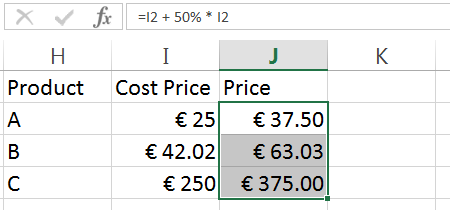
\includegraphics[height=3cm]{implementation/extractformula/21}
\subcaption{User selects formulas to be refactored}
\label{fig:extractformulaexample2a}

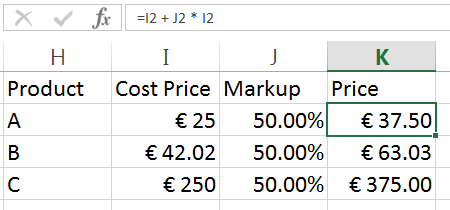
\includegraphics[height=3cm]{implementation/extractformula/23}
\subcaption{User selects formula to be extracted}
\label{fig:extractformulaexample2c}
\end{minipage}
\begin{minipage}[c][8cm][t]{0.5\textwidth}
\vspace*{\fill}
\centering
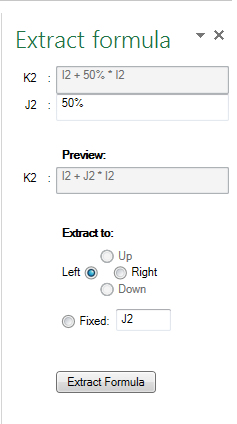
\includegraphics[height=7cm]{implementation/extractformula/22}
\subcaption{User selects formula to be extracted}
\label{fig:extractformulaexample2b}
\end{minipage}
\caption{An example application of \rf{Extract Formula}}
\label{fig:extractformulaexample2}
\end{figure}

The refactoring requires the user to select cell(s) to be refactored, type in the subformula to be extracted and select where the extraction should occur to.
Figure \ref{fig:extractformulaexample2} shows the process as experienced by the user.
The user first selects the formulas to be extracted (Figure \ref{fig:extractformulaexample2a}) and clicks the Extract Formula entry in the refactoring context menu (not shown).
A side-panel pops out which allows the user to enter the sub-formula to be extracted and where it should be extracted to (Figure \ref{fig:extractformulaexample2b}) and presses the Extract Formula button.
In the example the \f{50\%} subformula was extracted to the left, and Figure \ref{fig:extractformulaexample2c} shows the situation after the user has named the new column.

\todo{Nummering}

\subsection{Implementation}

Call the original formula $F_{or}$, the refactored formula $F_{new}$, the (user-supplied) subformula to be extracted $F_{sub}$.

If multiple cells are refactored at once, repeat the above process for all formulas.
Formulas with the same R1C1 $F_{or}$ have the same R1C1 $F_{new}$ so the intermediate steps of the process are cached.

\subsection{Detection of applicability}

Extract formula is always applicable to a formula cell, as even a very simple formula like \f{=1} still has a component that can be extracted.
In this case \f{=1} would become \f{=A1} and A1 would become \f{=1}.
Whether it is a good thing to perform the refactoring is of course the question, but the refactoring relies on the user to make this assessment.

\subsection{Improvements over RefBook \rf{Extract row or column} and \rf{Extract Literal}}
\label{subsubsec:improvementsextractformula}

Two specialized versions of this refactorings where previously described by Bamade and Dig \cite{badame2012refactoring} and implemented in their RefBook tool.
Their \rf{Extract Row or column} and \rf{Extract Literal} refactorings can both be performed by \rf{Extract formula}.

The author has chosen to not keep the \rf{extract row or column} refactoring name because it does not fully describe the refactoring (a full row or column does not necessarily have to be extracted) and to keep the name in line with refactorings in other domains.

The RefBook \rf{extract literal} refactoring can put a constant value into a cell and replace the occurrences of it with references to that cell, this is also possible with the BumbleBee \rf{extract formula} refactoring.
The BumbleBee \rf{Extract Formula} refactoring has several advantages over Badame's implementation of \rf{Extract row or column}.

Firstly RefBook does not handle operator precedence.
This can be very problematic for this refactoring and in the authors opinion should prevent is from being implemented, because one of the prime properties of a refactoring should be that it does not change the program results.
Note that the RefBook authors were aware of this deficiency, and left this as future work.
This future work has been performed by the thesis author.

Secondly RefBook can only handle a single row or column, which has to have exactly the same R1C1 formula. It can only extract the subformula to a column right of or row up of the original range.
BumbleBee can handle arbitrarily shaped ranges, with the only requirement that the subformula to be extracted occurs in all selected formulas.
Furthermore in addition to extracting to a cell neighboring the original formula cell (up, down, left or right) it can also extract the subformula to a single shared cell location.
This is very useful to remove duplication and makes the refactoring more universal by merging the \rf{extract literal} refactoring into it.

\section{\rf{Inline formula}}

\section{\rf{Introduce (Conditional) Aggregate}}

\section{\rf{Group References}}

\section{\rf{Fixate References}}

\todo{Unsure of ik deze nog wil implementeren, maar lijkt zeer laaghangend fruit.}

The Fixate References is similar to the \rf{Make Cell Constant} refactoring described by Badame \cite{badame2012refactoring}.
Maar beter want: user kan zelf selecteren welke cellen wel/niet absolute.

"Fixate references" beschrijft 100x beter wat de refactoring doet dan "Make cell constant". "Make cell constant" zou eerder impliceren dat je het resultaat van de cell berekening neemt en dat opslaat i.p.v. de formula. Wat trouwens ook weer een potentiele refactoring is, maar misschien een beetje een anti-pattern in excel.

\section{\rf{Introduce name}}

\todo{Kandidaat voor implementatie, meer laaghanged fruit.}

Cell (of range?) een naam geven, overal waar die naar gereferenced wordt vervangen door cell naam.
Of gelijk bij extract formula intregrereren!

\chapter{Evaluation}


\chapter{Conclusion}

\section{Future Work}

\bibliographystyle{unsrt}
\bibliography{thesis}

\appendix

\chapter{Code listings}

\lstset{style=sharpc}
\begin{lstlisting}[float,caption={XLParser Print method (simplified)}, label={lst:xlparserprint}]
public static string Print(this ParseTreeNode node) {
  // Print token values
  if(node is Terminal) return node.Token.Text;
  
  // Select is C#'s map function
  var ch = node.ChildNodes.Select(Print).ToList();
  
  switch(node.Type()) {
     case "ArrayFormula":
       return "{=" + ch[0] + "}";
     case "FunctionCall":
       if(node.IsBinaryOperation()) {
          return ch[0] + " " + ch[1] + " " + ch[2];
       }
       if(node.isNamedFunction()) {
          return String.Join("", ch) + ")";
       }
       // some more conditions
       break;
     // More cases for every node type
  }
}
\end{lstlisting}

\chapter{A Grammar for Spreadsheet Formulas Evaluated on Two Large Datasets}
\label{appendix:xlparser}

The following is a verbatim copy of the papers as it was published in the proceedings of SCAM 2015.

\clearpage

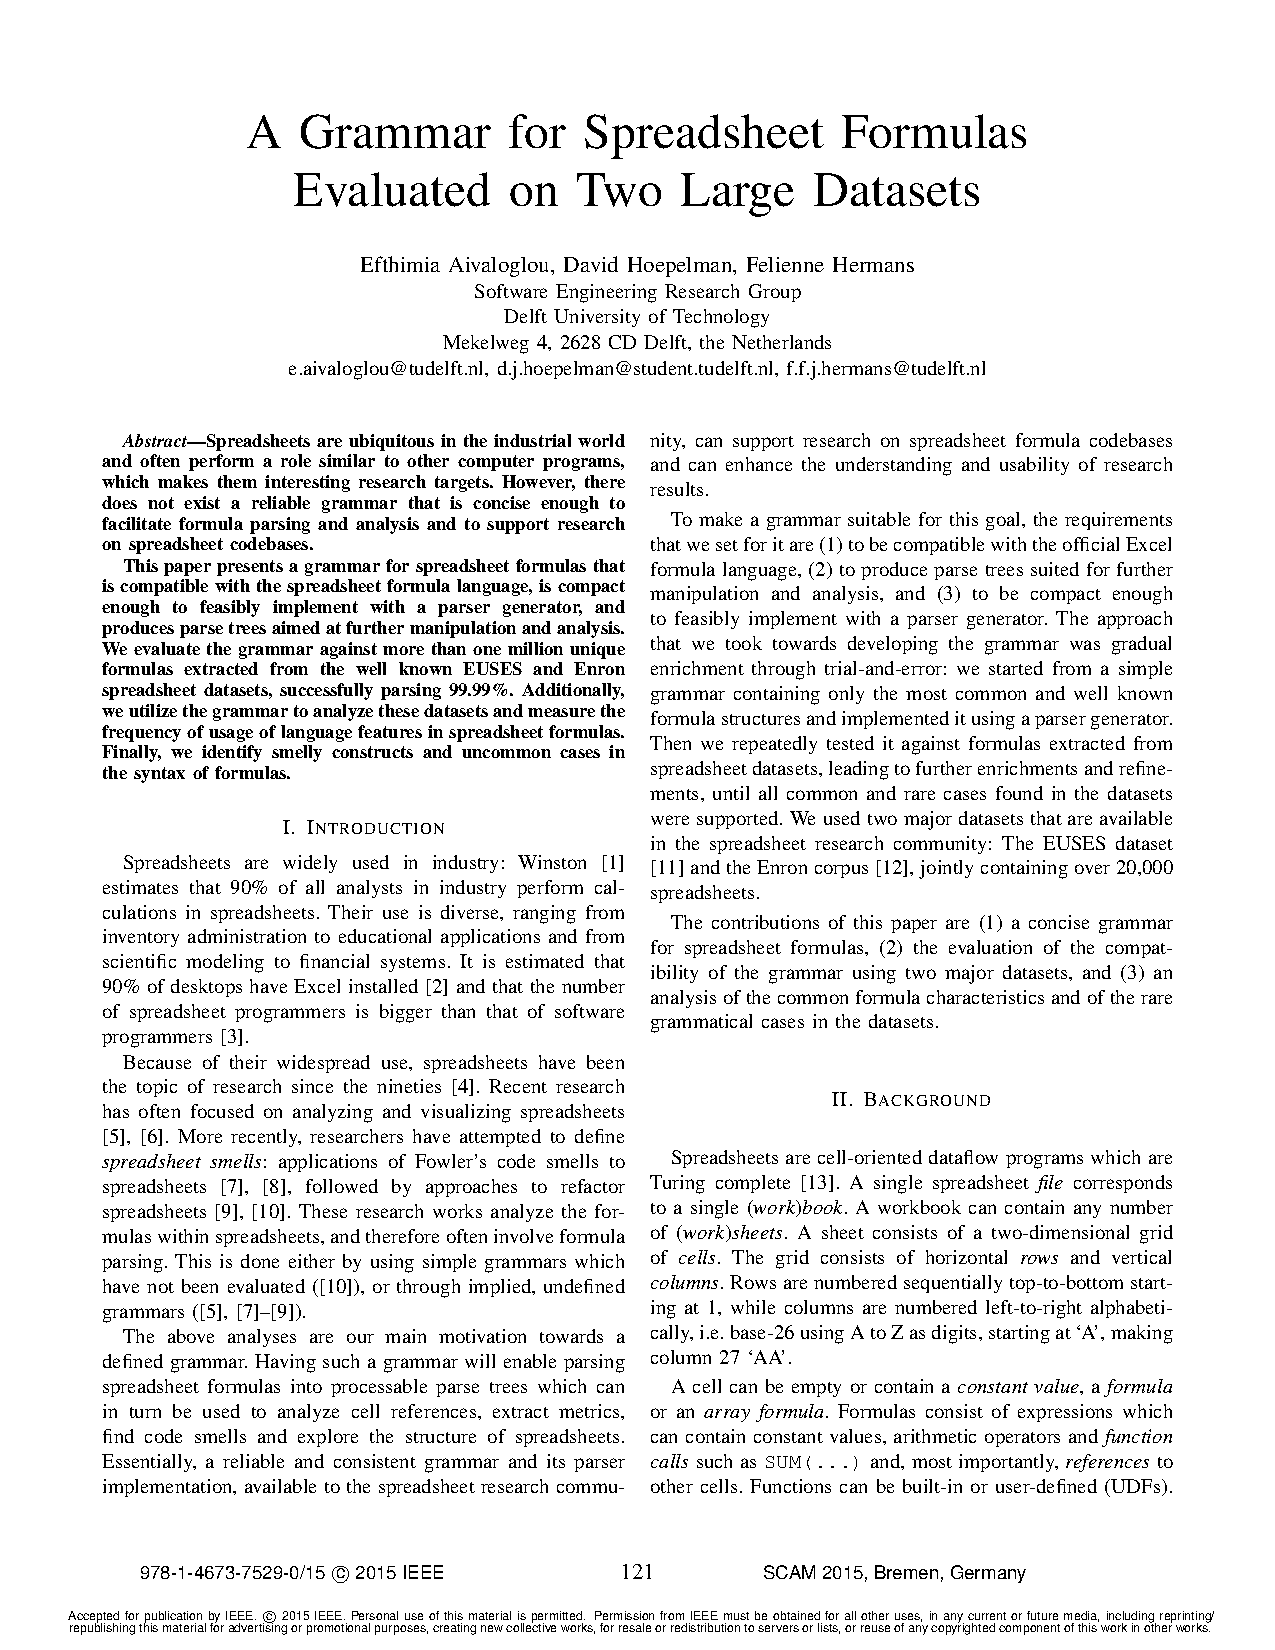
\includepdf[pages={1-10}]{appendix/scam-xlparser.pdf}

\clearpage

\vspace*{\fill}

\centering
\large{End of appendix \ref{appendix:xlparser}}

\vspace*{\fill}

\end{document}

